\chapter{Regression modeling with multiple predictors}





\section{Multiple predictor linear regression}

The real power of regression comes when we work with models of the form 
\begin{align}
Y &= b + \sum_{i=1}^K a_iX_i + \epsilon\\
\epsilon &\sim {\rm Normal}(0,\sigma_{\epsilon})
\end{align}
where $X_i$ is a set of $K$ predictor variables. If we want to think about this in terms of conditional averages, then 
\begin{equation}
Y|(X_1=x_1,\dots,X_K=x_K) \sim {\rm Normal}\left( b + \sum_{i=1}^K a_iX_i,\sigma_{\epsilon}\right)
\end{equation}

This is the simplest generalization of the single-predictor regression model to work with multiple predictors, although as we will see it is not the only generalization. We now want to answer all the questions we asked for the original regression model in the context of this model, such as: 
\begin{enumerate}
\item What assumptions are we making and how do we interpret the parameters $a_i$? 
\item What are estimators of the parameters from data? 
\item How accurate is our model at predicting new $Y$ values based on $X$ values? 
\end{enumerate}



\subsubsection{Multiple predictors in python}
Let's start by seeing how to work with multiple predictors in python
The first step is to get the predictor variables in the correct format for statsmodels. Statsmodels wants us to input a multidimensional arrray 
\begin{equation}
X = \left[\begin{array}{ccc}
1 &x_{1,1}& x_{1,2}\\
1 &x_{2,1}& x_{2,2}\\
\vdots & \vdots & \vdots\\
1 &x_{n,1}& x_{n,2}\\
\end{array} \right]
\end{equation}

The $i$th column contains the predictors that go with our $i$th observation $y$. This will tell statsmodels to also include a constant term (the intercept) $\beta_0$ in our regression. 

The following code will get our data in this format:
\begin{Verbatim}
X = sm.add_constant(np.transpose(np.array([x_hs,x_iq])))
\end{Verbatim}

\begin{example}
\href{https://colab.research.google.com/drive/1oIRgP_7-c5DGV1D2iz5nj406mZfJxUIG#scrollTo=wbeO1TS8os5J&line=15&uniqifier=1}{Our first regression with multiple predictors}
\end{example}

%\begin{example}
%\href{}{Our first regression with multiple predictors}
%\end{example}

\section{Interpretation and estimation of the parameters }

In order to interpret the parameters, it's easiest to work with just two predictors:
\begin{equation}
Y = b + a_1X_1 + a_2X_2 + \epsilon.  
\end{equation}
Let start by just looking at the deterministic equation:  
\begin{equation}
y = b + a_1x_1 + a_2x_2
\end{equation}
This describes a flat surface in two dimensions as shown in Figure \ref{fig:plane}

\begin{figure}[h]
    \centering
    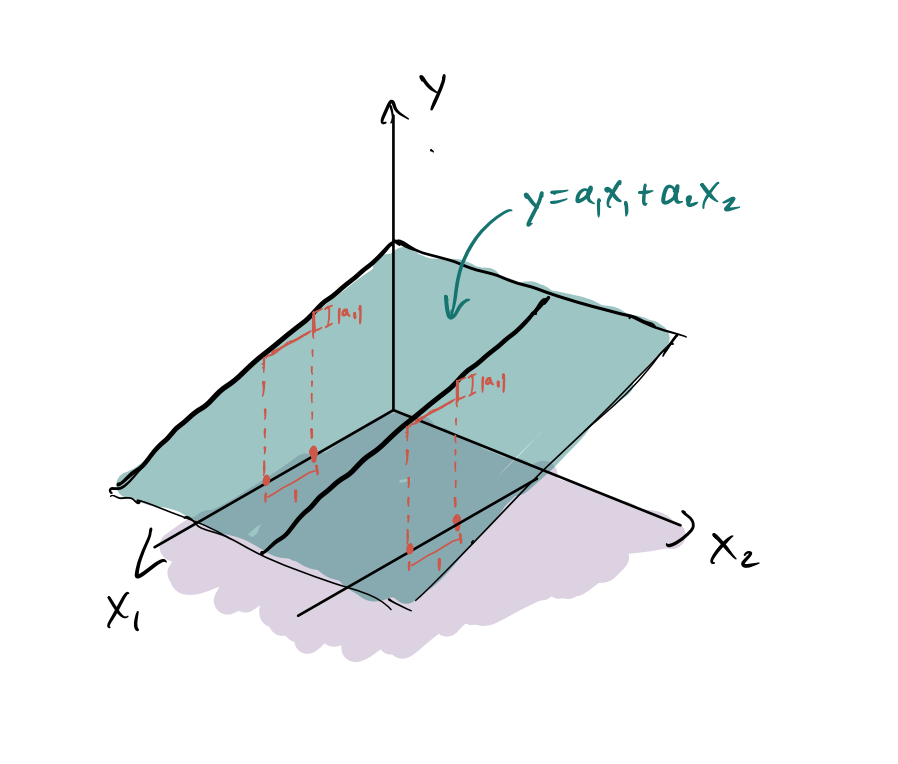
\includegraphics[width=0.8\textwidth]{plane}
    \caption{The function $y(x_1,x_2)$}
    \label{fig:plane}
\end{figure}


 If we make a slide through the surface in the $x_1$ direction and look it at from the side, we see a line with slope $a_1$ (and similarly for $x_2$).  Now back to the regression model. We can understand $a_1$ is the slope of $Y$ vs. $X_1$ for fixed (conditioned on) $X_2$. 
 {\bf The fact that it doesn't matter which value of $X_2$ we condition is an assumption of the model}.  Mathematically, we can write
 \begin{equation}
 a_1 = \E[Y|X_1 = (x+1),X_2] -  \E[Y|X_1 = x,X_2].
 \end{equation}
 It is important that we condition on BOTH variables? 
 
  You might guess the coefficient $a_1$ is also ${\rm cov}(Y,X_1)/\sigma_{x_1}^2$. After all, if we look a slice of the 2D planer function $y(x_1,x_2)$ along the $x_1$ direction, we get the same slope for all $x_2$.  It stands to reason if we look at only the points in the $x_1$-$y$ plane our regression slope would be $a_1$. {\bf This argument assumes that when we change $x_1$, $x_2$ does not also change}. This is best understood with an example
  
  \begin{example}
\href{https://colab.research.google.com/drive/1oIRgP_7-c5DGV1D2iz5nj406mZfJxUIG#scrollTo=wbeO1TS8os5J&line=15&uniqifier=1}{Understanding the multiple predictors regression slopes}
\end{example}
  
The important thing is that when we increase $x_1$ we are ALSO increasing $x_2$. 


\begin{figure}[h]
    \centering
    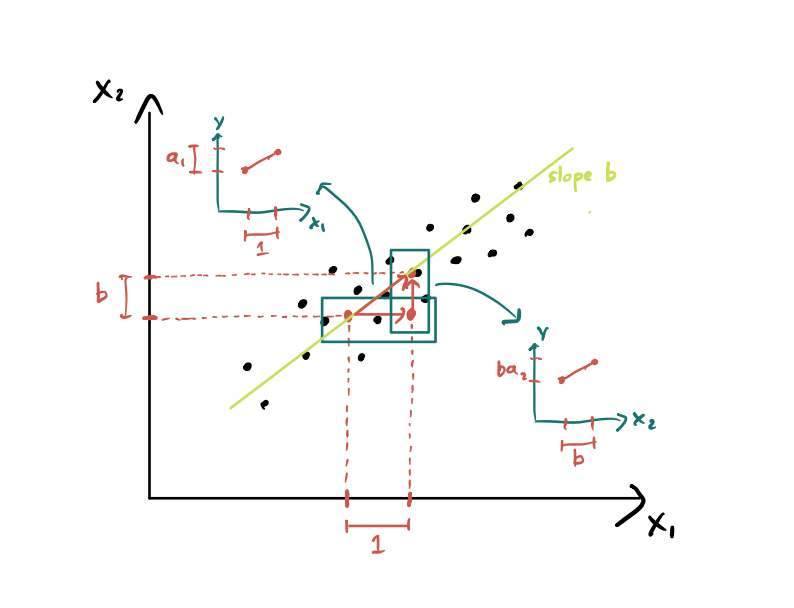
\includegraphics[width=0.8\textwidth]{correlated_predictors}
    \caption{When we increase $x_1$ by $1$, $x_2$ changes by $b$ (which is the slope between $x_1$ and $x_2$ here, not the intercept.) }
    \label{fig:plane}
\end{figure}



If the usual relationship in terms of the covariance doesn't hold, is there a more general relationship expression for $a_1$ in terms of conditional averages. The answer is, of course, yes! To get there, we need to us some linear algebra which is beyond the scope of these notes. If you are interested, it goes something like this: 
\begin{align}
\left[\begin{array}{c}
a_1 \\
a_2 
\end{array}\right] &= \left[\begin{array}{cc}
\sigma_{x_1}^2 & {\rm cov}(X_1,X_2)\\
 {\rm cov}(X_1,X_2) & \sigma_{x_2}^2
 \end{array} \right]^{-1}\left[ \begin{array}{c}
 {\rm cov}(X_1,Y)\\
  {\rm cov}(X_2,Y)\\
  \end{array}\right]\\
  &=  \frac{1}{\sigma_{x_2}^2\sigma_{x_1}^2 -{\rm cov}(X_1,X_2)^2} \left[\begin{array}{cc}
\sigma_{x_2}^2 & -{\rm cov}(X_1,X_2)\\
- {\rm cov}(X_1,X_2) & \sigma_{x_1}^2
 \end{array} \right]\left[ \begin{array}{c}
 {\rm cov}(X_1,Y)\\
  {\rm cov}(X_2,Y)\\
  \end{array}\right]
%  &=\left[\begin{array}{c}
%   \frac{ {\rm cov}(X_1,Y)\sigma_{x_2}^2 - {\rm cov}(X_2,Y){\rm cov}(X_1,X_2)}{\sigma_{x_2}^2\sigma_{x_1}^2 -{\rm cov}(X_1,X_2)^2}\\
%     \frac{ {\rm cov}(X_2,Y)\sigma_{x_1}^2 - {\rm cov}(X_1,Y){\rm cov}(X_1,X_2)}{\sigma_{x_2}^2\sigma_{x_1}^2 -{\rm cov}(X_1,X_2)^2}
%  \end{array}
%  \right]
\end{align}
After using the formula for the inverse of $2\times 2$ matrix, we obtain 
\begin{align}
a_1 &=     \frac{ {\rm cov}(X_1,Y)\sigma_{x_2}^2 - {\rm cov}(X_2,Y){\rm cov}(X_1,X_2)}{\sigma_{x_2}^2\sigma_{x_1}^2 -{\rm cov}(X_1,X_2)^2}\\
&= \frac{ {\rm cov}(X_1,Y)- {\rm cov}(X_2,Y){\rm cov}(X_1,X_2)/\sigma_{x_2}^2 }{\sigma_{x_1}^2 -{\rm cov}(X_1,X_2)^2/\sigma_{x_2}^2 }
\end{align}
You don't need to worry about this formula, but it essentially tells us how $a_1$ can be estimated from data: We replace the covariances and variances with the corresponding sample averages.  Notice that if all the variances are equal to one: 
\begin{equation}
a_1 = \frac{1}{1-\rho_{1,2}}(\rho_1 - \rho_{1,2}\rho_2)
\end{equation}
where $\rho_{1,2}$ is the correlation coefficient between $X_1$ and $X_2$. Notice that if $X_1$ and $X_2$ are uncorrelated ($\rho_{1,2}=0$), we obtain the usual connection between the regression coefficient and the correlation coefficient between $X_1$ and $X_2$. 
%
%
%This is not the same as the regression slope of $Y$ vs. $X_1$. Why? 
%\begin{align}
%\tilde{a}_1 &= \E[Y|X_1=(x+1)] -  \E[Y|X_1=x] \\
%&= a_1+ \underbrace{a_2( \E[X_2|X_1=(x+1)]- \E[X_2|X_1=x])}_{=\delta_{1,2}}
%\end{align}
%The second contribution $\delta_{1,2}$ characterizes the change in slope as a result of a bias towards higher or lower values of $x$. Notice that, if we were to model for $X_2$ vs $X_2$ with slope $u$, then 
%\begin{equation}
%\delta_{1,2} = a_2u
%\end{equation}
%We can understand this geometrically if we visualize the $X_2$ vs. $X_1$ plain from above. 
%

\begin{exercise}
\href{https://colab.research.google.com/drive/1oIRgP_7-c5DGV1D2iz5nj406mZfJxUIG#scrollTo=wbeO1TS8os5J&line=15&uniqifier=1}{Test score data}
\end{exercise}


\begin{exercise}
\href{https://colab.research.google.com/drive/1oIRgP_7-c5DGV1D2iz5nj406mZfJxUIG#scrollTo=wbeO1TS8os5J&line=15&uniqifier=1}{More on test scores}
\end{exercise}


This can all be generalized to the situation where we have many predictors. The general formula for the regression coefficient would be: 
\begin{align}
\begin{split}
a_i &= \E[Y|X_1,\dots,X_{i-1},X_i=x_i+1,X_{i+1},\dots,X_K]\\
&\quad\quad - \E[Y|X_1,\dots,X_{i-1},X_i=x_i,X_{i+1},\dots,X_K]
\end{split}
\end{align}
We get a more complex expression for the coefficients but the idea is the same. 



\section{Collinearity and sloppy models}

\subsection{The sample distribution of coefficients}
Just as before, we want to understand what the sample distribution of the coefficients looks like. In the multiple predictor case, this becomes more interesting, as the following example illustrates. 


\begin{figure}[h]
    \centering
    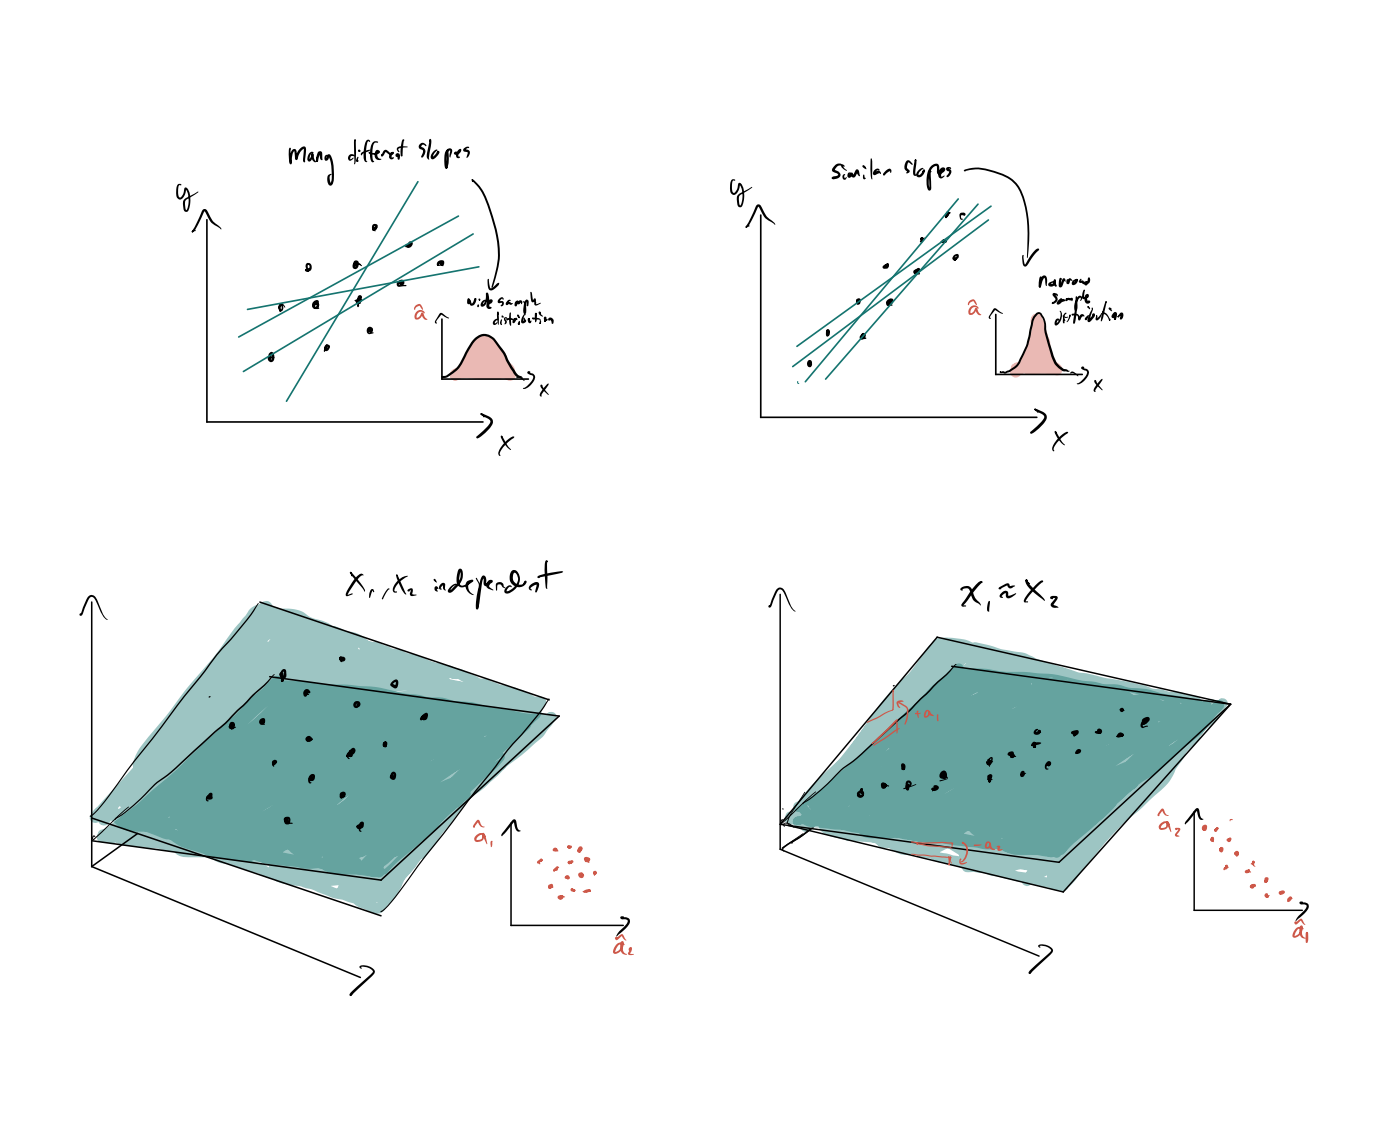
\includegraphics[width=0.8\textwidth]{sample_dist}
    \caption{(top) In the single-predictor case, the width of the sample distribution measures how confident we are of a particular slope. It will be narrow if a replicate of our data is likely to produce a very similar slope.  These means we get a rough idea of the width of sample distribution by seeing much we can change our regression line and still obtain something that appears to pass through our data. (bottom) In the two predictor case, we have a regression plane and changing $a_1$ and $a_2$ will ``wiggle" the plane by tilting it in the $x_1$ and $x_2$ directions (there is also the intercept which can shift the plane up and down, but I'm not illustrating that). If $X_1$ and $X_2$ are uncorrelated, it doesn't matter which way we wiggle it, the fit will be similar, but if $X_1$ and $X_2$ are strongly correlated, wiggling the plane in the direction perpendicular  to the points has a much smaller effect that parallel to them. }
    \label{fig:sample_dist}
\end{figure}



\begin{example}
\href{https://colab.research.google.com/drive/1oIRgP_7-c5DGV1D2iz5nj406mZfJxUIG#scrollTo=h_vbLZqWPNzD&line=1&uniqifier=1}{Understanding multivariate sample distribution}
\end{example}


To better understand what is going on, imagine $X_1$ and $X_2$ are very highly correlated (if they are perfectly correlated we say they are {\dfn colinear}). We can then write 
\begin{align}
Y &= a_1X_1 + a_2X_2 + \epsilon  \approx a_1X_1 + a_2X_1 + \epsilon\\
 &\approx (a_1+a_2)X_1 + \epsilon
\end{align}
There are many ways to select $a_1$ and $a_2$ so that the surface $a_1x_1+a_2x_2$ is close to the lines, since a change in $a_1$ can be compensated by a change in $a_2$. This means that {\bf if we estimate $a_1$ and $a_2$ and then generated new data, it would be possible to get a VERY different value of $\hat{a}_1$ and $\hat{a}_2$, so long as $\hat{a}_1 + \hat{a}_2$ is close to what we got before}. This is illustrated in Figure \ref{fig:sample_dist} and Figure \ref{fig:sample_dist2}. The following exercises explored in more depth what this means for the sample distribution. 

\begin{figure}[h]
    \centering
    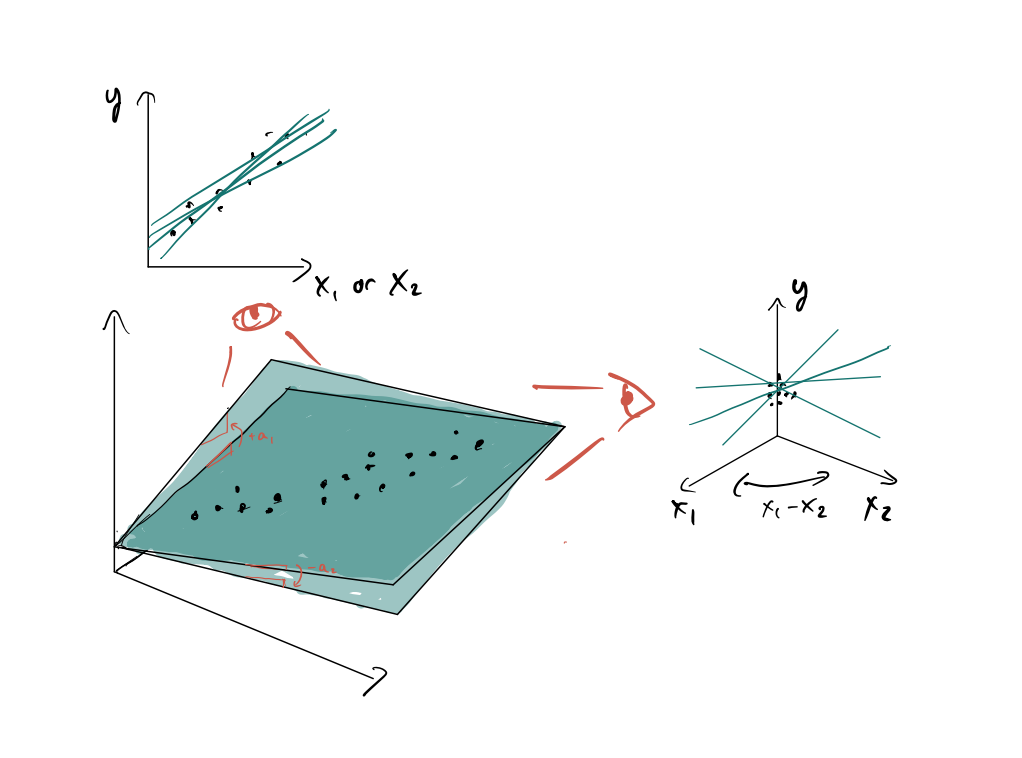
\includegraphics[width=0.8\textwidth]{sample_dist2}
    \caption{Different views of the data in the case when $X_1$ and $X_2$ are correlated. If we look at the data from the side, or along the $X_1=X_2$ direction, then all our regression planes appear similar; however, when looked at from the ``front" as shown in the right panel, we see that the places actually have very different slopes in the other direction.  }
    \label{fig:sample_dist2}
\end{figure}




\begin{exercise}
\href{https://colab.research.google.com/drive/1oIRgP_7-c5DGV1D2iz5nj406mZfJxUIG#scrollTo=h_vbLZqWPNzD&line=1&uniqifier=1}{Understanding multivariate sample distribution}
\end{exercise}

\begin{exercise}
\href{https://colab.research.google.com/drive/1oIRgP_7-c5DGV1D2iz5nj406mZfJxUIG#scrollTo=SugKDnavWgtU&line=3&uniqifier=1}{Sample distributions and predictors}
\end{exercise}

\begin{exercise}
\href{https://colab.research.google.com/drive/1oIRgP_7-c5DGV1D2iz5nj406mZfJxUIG#scrollTo=SugKDnavWgtU&line=3&uniqifier=1}{Implications for predictions}
\end{exercise}

\subsection{Changing variables. }  
At this point, you should understand that the sample distribution is related to correlations between $x_1$ and $x_2$. Indeed, for a large enough sample, one can show that
\begin{equation}
\hat{a}_1 \sim {\rm Normal}\left( a_1,\sqrt{ \frac{\sigma_{\epsilon}^2\sigma_{x_1}^2}{{ \rm cov}(X_1,X_2)^2 -\sigma_{x_1}^2\sigma_{x_2}^2 }}\right)
\end{equation} 
Here, we can see explicitly what happens when $X_1$ and $X_2$ become highly correlated -- the standard deviation of the sample distribution blows up. When this happens, we will say the model is {\dfn sloppy}. How do we deal with this situation? One approach is to use different predictor variables, for example, if $X_1 \approx X_2$, we might simply work with $X_1 + X_2$ as our predictor.




\section{Dealing with categorical data}
One situation in which models with multiple predictors frequently arrises is when trying to predict a $Y$ variable based on categorical predictors, such as race. In this case, we need to transform the categories  into numerical values. For example, if there are two cataogies, we map our variable to $0$ or $1$. If we have $3$ categories, we might first think to map them to $0$, $1$ and $2$. This has a problem though: A chance from $1$ to $2$ should not necessarily  correspond to a change from $0$ to $1$. {\bf There is no ordering of the $x$ values}. Thus, instead we introduce a new variable, which is 1 if our data point is in the third category and zero otherwise. Do you see what the problem would be if we have $3$ $X$ variables, one for each category? 

In order to take a categorical variable and transform it into a set of indicator variables in python, we use 
\begin{Verbatim}
get_dummies
\end{Verbatim}


\begin{example}
\href{https://colab.research.google.com/drive/1oIRgP_7-c5DGV1D2iz5nj406mZfJxUIG#scrollTo=wbeO1TS8os5J&line=15&uniqifier=1}{Working with categorical data}
\end{example}


\begin{exercise}
\href{https://colab.research.google.com/drive/1oIRgP_7-c5DGV1D2iz5nj406mZfJxUIG#scrollTo=wbeO1TS8os5J&line=15&uniqifier=1}{Understanding marginal regression coefficients}
\end{exercise}



\begin{exercise}
\href{https://colab.research.google.com/drive/1oIRgP_7-c5DGV1D2iz5nj406mZfJxUIG#scrollTo=wbeO1TS8os5J&line=15&uniqifier=1}{Simpson's paradox}
\end{exercise}

